%
% imagens.tex
%
% Workshop de LaTeX do SciELO
%
% Demonstra:
% - Como incluir gráficos com o pacote graphicx
% - Controlar o tamanho e escala dos gráficos
% - O ambiente figure
% - O ambiente minipage e seus usos
% - Outras capacidades do graphicx (ver documentação)
%

\documentclass[a4paper,oneside]{article}
\usepackage{fontspec}
\usepackage{polyglossia}
  \setdefaultlanguage{brazil}
\usepackage{graphicx}

\begin{document}
\frenchspacing

% Informação e imagem encontrados na Wikipédia em:
% https://en.wikipedia.org/wiki/Alpha_Centauri
\section{Nosso vizinhos}

Na figura~\ref{fig:estrelas}, podemos ver nossos vizinhos mais próximos, por
assim dizer. A estrela circulada é Proxima Centauri, uma pequena anã vermelha,
que pode estar ligada gravitacionalmente às outras duas estrelas. A olho nu, as
duas estrelas parecem uma só.

% Brincar os as opções de posicionamento do figure e de tamanho do
% \includegraphics. Ensinar o ambiente minipage, e a técnica de colocar dois
% minipages dentro de um figure para colocar uma imagem ao lado da outra.
\begin{figure}[h]
  \centering
  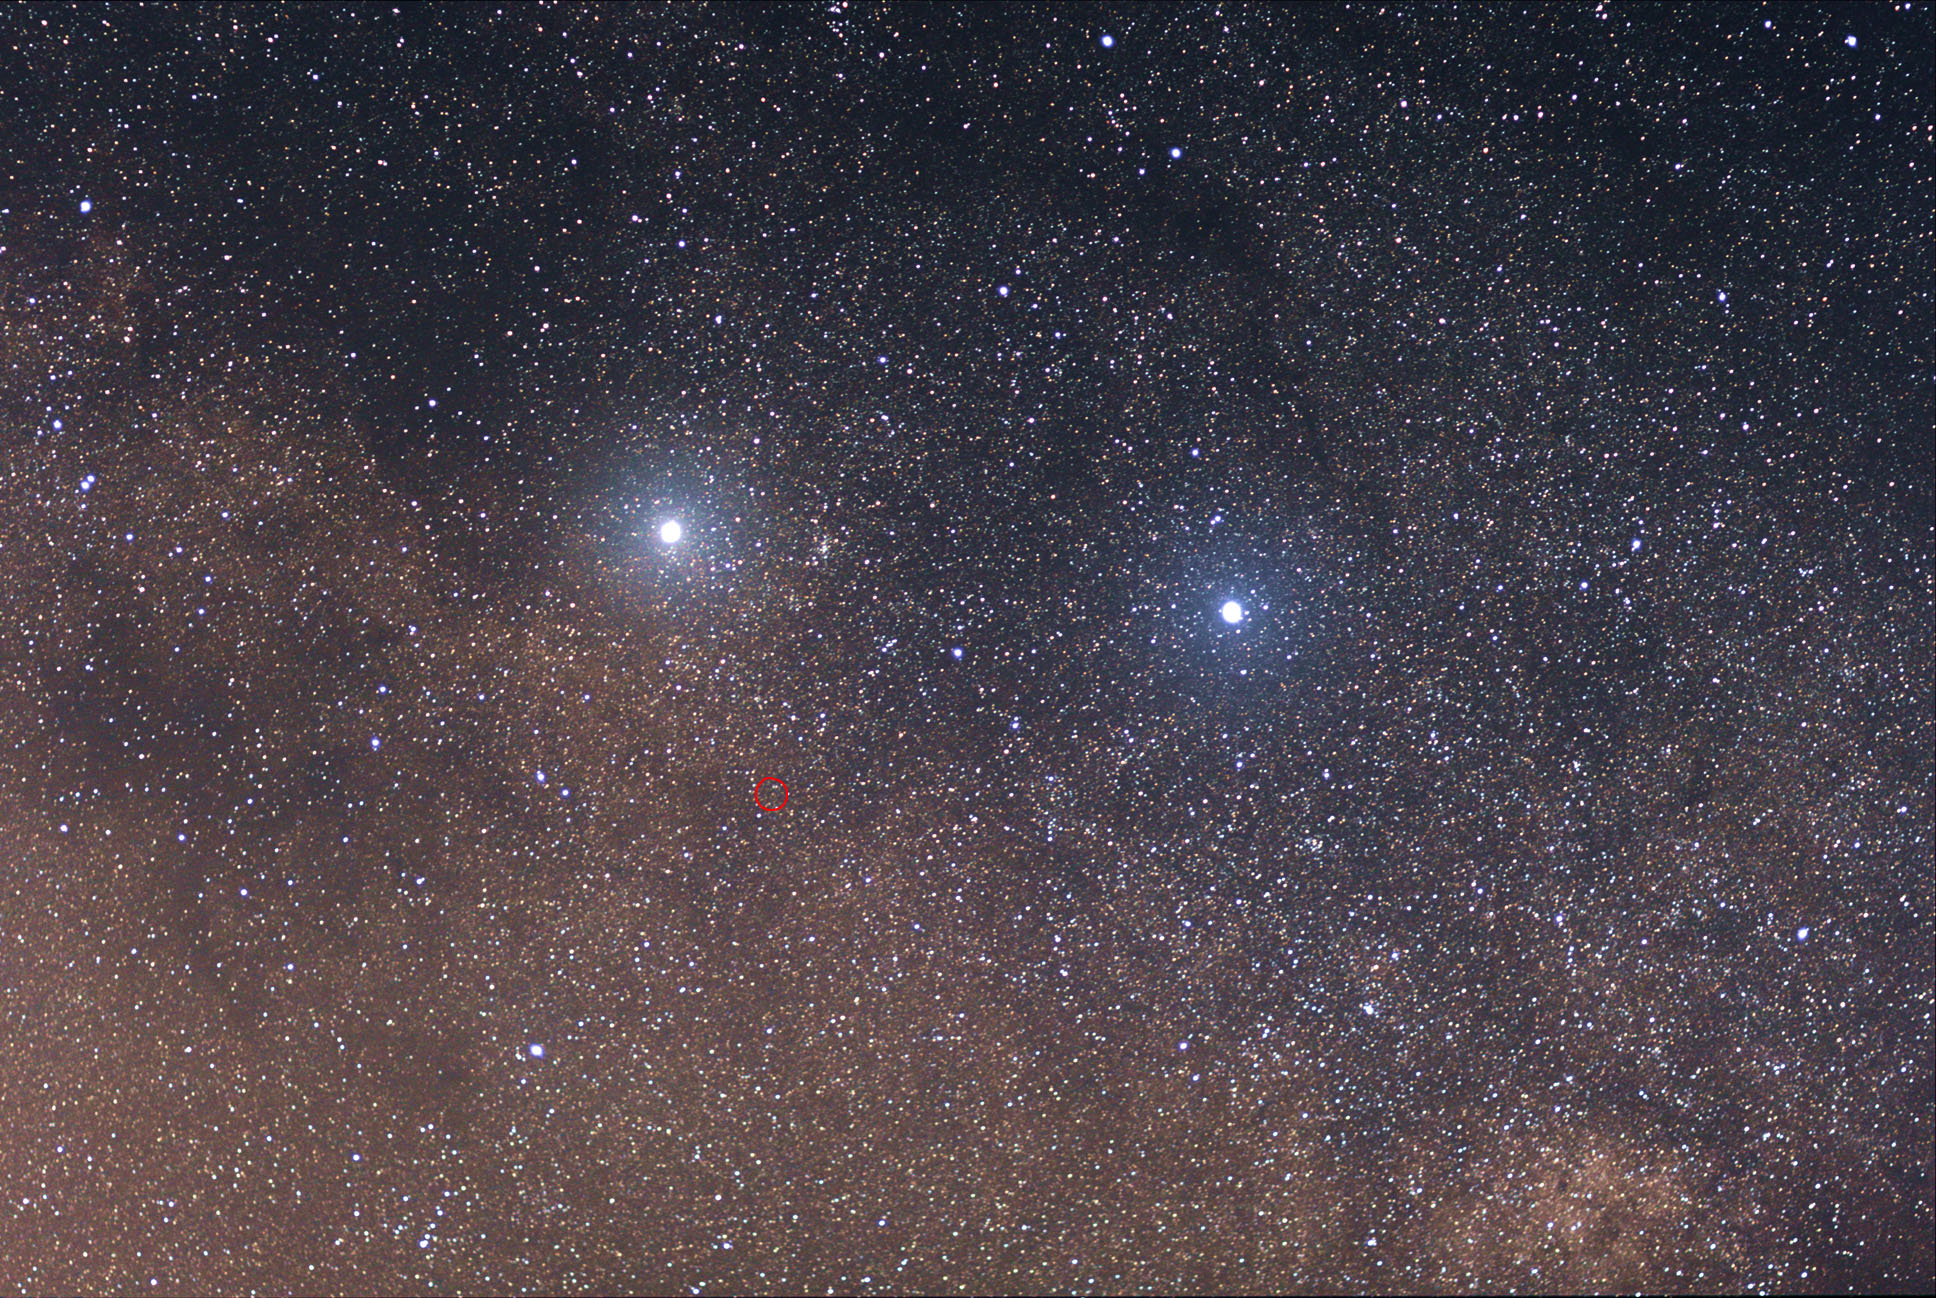
\includegraphics[width=\textwidth]{imagens/alpha-beta-proxima-centauri}
  \caption{Alpha Centauri e Beta Centauri, com Proxima circulada}
  \label{fig:estrelas}
\end{figure}
\end{document}
